\section{Statistic for data science}

\subsection{Theory}

\subsubsection{Lecture 1}

Statistics is the approach of answering questions using data. We aim to find rules that are true for a certain population basing our findings on a smaller subset of the mentioned population (sample)

\vspace{10pt}

\textbf{Unit} $\xrightarrow{}$ Basic objrcts on which the data are collected

\textbf{Variable} $\xrightarrow{}$ Characteristics of units that can take different values

\vspace{10pt}

We can have different types of variables
\vspace{10pt}

\textbf{Categorical}
\begin{itemize}
    \item Nominal
    \item Ordinal
\end{itemize}

\textbf{Quantitative}
\begin{itemize}
    \item Discrete
    \item Continuous
\end{itemize}

Our questions involve large \textbf{populations}. Since we can't measure all of the units of them we usually take a subset called \textbf{sample}. Values that concern the sample are called \textbf{statistics} while the ones that concern the whole population are called \textbf{parameters}. 

\vspace{10pt}

We want to estimate in a precise way those parameters basing the computation on the sample.

One of the problems regarding the samples is that those can be biased. To avoid that we want to get a sample that is representative of the population. One way is the use of \textbf{simple random sampling method}.

\textbf{Describing and visualizing data}

We have different ways to describe our data, they depend on multiple factors.

Categorical variables can be described by a proportion



\[
p = \frac{\text{Number in the category}}{\text{Total number}}
\]

To assess how many units share a certain value we can use a \textbf{Bar chart}

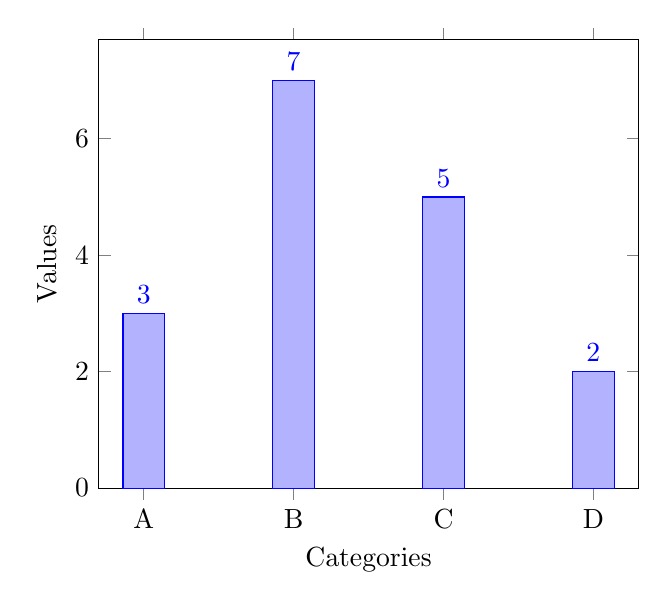
\begin{tikzpicture}
  \begin{axis}[
      ybar,
      bar width=15pt,
      xlabel={Categories},
      ylabel={Values},
      symbolic x coords={A,B,C,D},
      xtick=data,
      nodes near coords, % mostra i valori sopra le barre
      ymin=0,
  ]
    \addplot coordinates {(A,3) (B,7) (C,5) (D,2)};
  \end{axis}
\end{tikzpicture}

\vspace{10pt}

One important concept in statistics is central tendency, which refers to finding the center of our data. It also helps us understand how the other values are distributed around that center. Quantitative variables can be summarized using measures of central tendency.

\vspace{10pt}

\textbf{Mean} $\xrightarrow{}$ Sum of the data values divided by the number of the values. For the mean of the sample we use $\bar{x}$ and for the one of the population $\mu$. The formula is

\[
\bar{x} = \frac{1}{n} \sum_{i=1}^n x_i
\]

\vspace{10pt}

\textbf{Median $\xrightarrow{}$} The center of sample after it was ordered from smallest to largest. Better than mean if we have outliers.

\vspace{10pt}

\textbf{Standard deviation} $\xrightarrow{}$ It describes how the units are distributed from the mean. We can square it to get the variance. For the sample we call it $s$, for the population we use $\sigma$. 

\[
s = \sqrt{\frac{1}{n-1} \sum_{i=1}^n (x_i - \overline{x})^2}
\]

Remember that both $\bar{x}$ and $s$ (or $s^2$) are relative to the sample. They are just an estimation that might be correct if we have a big enough sample.

\vspace{10pt}

\textbf{Percentile} $\xrightarrow{}$ Is a measure that tells us the percentage of the observations that fall at or below it. At $75\%$ we will find on the left the 75\% of the observations and on the right the 25\%.

\vspace{10pt}


\textbf{Quartiles} $\xrightarrow{}$ Basically the same as the percentiles but now we are dividing the sample in 4 parts. $Q_1$ is the first quartile, we will find on the left 25\% of the observations and the rest on the right. $Q_2$ is the median.

\[
Q_1 = \text{25th percentile}, \quad
Q_2 = \text{median (50th percentile)}, \quad
Q_3 = \text{75th percentile}
\]

\[
\text{Interquartile Range (IQR)} = Q_3 - Q_1
\]

\[
\text{Lower fence} = Q_1 - 1.5 \cdot \text{IQR}, \quad
\text{Upper fence} = Q_3 + 1.5 \cdot \text{IQR}
\]

\[
\text{Outliers} = \text{values outside } [\text{Lower fence}, \text{Upper fence}]
\]

\vspace{10pt}

We can visualize those statistics using a \textbf{Boxplot}

\begin{tikzpicture}
\begin{axis}[
    boxplot/draw direction=y,
    ylabel={Values},
    xtick={1},
    xticklabels={Sample Data},
    width=8cm,
    height=6cm
]

% boxplot principale
\addplot+[
    boxplot prepared={
        median=50,
        upper quartile=60,
        lower quartile=40,
        upper whisker=80,
        lower whisker=20
    },
] coordinates {};

% outlier come punti separati
\addplot+[
    only marks,
    mark=*,
    mark options={red},
] coordinates {(1,10) (1,15) (1,90) (1,95)};

\end{axis}
\end{tikzpicture}



\vspace{10pt}

\textbf{Correlation} $\xrightarrow{}$ Describes the strength and direction between two quantitative variables. For the sample we use $r$, for the population we use $\rho$.

\vspace{10pt}

Correlation has many properties:
\begin{enumerate}
    \item $\rho$ is bounded in [-1, 1]
    \item $\rho$ > 0 means positive association, $\rho$ < 0 negative, $\rho$ = 0 no relationship
    \item The bigger |$\rho$| the stronger the correlation
    \item The sign tells the direction
    \item $\rho$ is unit free
    \item $\rho$(X, Y) = $\rho$(Y, X)
    
\end{enumerate}

To visualize correlation we use a \textbf{Scatterplot}


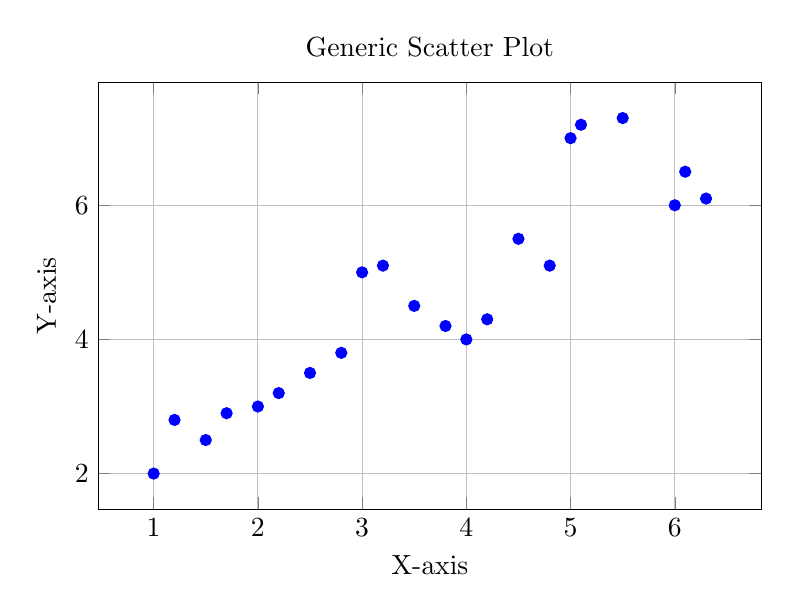
\begin{tikzpicture}
  \begin{axis}[
      xlabel={X-axis},
      ylabel={Y-axis},
      title={Generic Scatter Plot},
      width=10cm,
      height=7cm,
      grid=major,
  ]
    % Dati del scatter plot
    \addplot[
      only marks,
      mark=*,
      mark size=2pt,
      color=blue
    ] coordinates {
        (1,2) (2,3) (3,5) (4,4) (5,7) (6,6)
        (1.5,2.5) (2.5,3.5) (3.5,4.5) (4.5,5.5)
        (1.2,2.8) (2.2,3.2) (3.2,5.1) (4.2,4.3)
        (5.1,7.2) (6.3,6.1) (1.7,2.9) (2.8,3.8)
        (3.8,4.2) (4.8,5.1) (5.5,7.3) (6.1,6.5)
    };
  \end{axis}
  
\end{tikzpicture}

\hrule

\subsubsection{Lecture 2}

\vspace{10pt}

Since random variables can take certain values with certain probabilities we would like to describe them somehow. The collection of those probability is called probability distribution. This can describe the probability of each event happening. Recall that the sum of the probabilities is 1.

\vspace{10pt}

\textbf{CDF} -> the \textbf{cumulative distribution function} gives me the probability that a random variable is less than or equal to a given value. 

\begin{equation}
    F(x) = P(X \le x) \quad \text{for all } x
\end{equation}


\textbf{PMF/PDF} -> the \textbf{probability mass function} or \textbf{probability density function} (for discrete or continuous case respectively) will give us the probability of a certain event happening

\begin{equation}
    f(x) = P(X = x), \quad \text{for all } x
\end{equation}

\begin{equation}
F(x) = \int_{-\infty}^{x} f(t)\,dt, \quad \text{for all } x
\end{equation}

For the continuous case we calculate the integral between the 2 values that we care 

\vspace{10pt}

\textbf{Discrete distributions}

If we can count the sample space we say that our random variable is discrete

Recall

\begin{equation}
    Var[X] = E[X^2] - E[X]^2
\end{equation}

\vspace{20pt}

\textbf{Bernoulli} -> the probability that a certain event will happen

\begin{equation}
    X \sim Ber(p)
\end{equation}
\begin{equation}
    P(X=1) = p = 1 -P(X=0) = 1-q
\end{equation}

With PMF

\begin{equation}
    f(x) = p^x(1-p)^x \quad \text{for x} \in \{0, 1\}
\end{equation}

Where

\begin{itemize}
    \item p -> positive probability
    \item q -> negative probability, 1-p basically
\end{itemize}

And with
\begin{itemize}
    \item E[X] = p
    \item Var[X] = pq = p(1-p)
\end{itemize}


\textbf{Binomial} -> probability of getting a certain number of getting n independent Bernoulli outcome

\begin{equation}
    X \sim Bin(n, p)
\end{equation}

\begin{equation}
    P(X=x) = \binom{n}{x}p^x(1-p)^{n-x}
\end{equation}

Where
\begin{itemize}
    \item n -> number of trials
    \item p -> positive probability
    \item x -> successes that we want to calculate
\end{itemize}

Recall that

\begin{equation}
    \binom{n}{x} = \frac{n!}{x!(n-x)!}
\end{equation}

And with
\begin{itemize}
    \item E[X] = np
    \item Var[X] = np(1-p)
\end{itemize}


\textbf{Poisson} -> probability of getting a certain number of events during a fixed interval. We need to know the probability of the event happening.

\begin{equation}
    X \sim Poi(\lambda)
\end{equation}

\begin{equation}
    f(x) = P(X=x) = \frac{\lambda^xe^{-\lambda}}{x!}
\end{equation}

Where

\begin{itemize}
    \item e -> Euler number
    \item x -> number of successes
    \item $\lambda $ -> known mean rate
\end{itemize}

With
\begin{itemize}
    \item E[X] = Var[X] = $\lambda$
\end{itemize}

\subsubsection{Lecture 3}

\textbf{Continuous distributions}

\vspace{10pt}


\textbf{Normal distribution} -> If we want to describe a series of random events that have a tendency of being near a certain mean.

\begin{equation}
    X \sim N(\mu, \sigma^2
\end{equation}

\begin{equation}
    \phi (x) = \frac{1}{\sqrt{2\pi\sigma^2}} \exp{\{-\frac{1}{2\sigma^2} (x-\mu)^2\}}
\end{equation}

\begin{itemize}
    \item E[X] = $\mu$
    \item Var[X] = $\sigma^2$
\end{itemize}

It has a bell shape and if the parameter are $\mu$ = 0 and $\sigma^2$ = 1 we say that is a standard normal distribution known as Z distribution. $\sigma^2$ will tell us how thin or wide is the distribution, so how variable it is, and so how unpredictable. 

Kurtosis -> Measure of how heavy the tails are, how frequent are the outliers

\vspace{10pt}

\vspace{10pt}

\textbf{Chi squared} -> If we have n independent X variables that are distributed with the Z distribution if we square and sum them we say that this quantity follows a Chi-squared distribution

\begin{equation}
    V=X_1^2+X_2^2+...+X_n^2 \sim\chi_{(n)}^2, n>0
\end{equation}

With
\begin{itemize}
    \item E[V] = n
    \item Var[V] = 2n
\end{itemize}

The n parameter is called \textbf{degrees of freedom}. The shape is asymmetric

\vspace{10pt}


\textbf{Student’s t distribution} $\rightarrow$  
If we have a random variable $Z$ distributed as a standard normal distribution and another independent variable $V$ following a Chi-squared distribution with $n$ degrees of freedom, then the following ratio defines a random variable that follows a t-distribution:

\begin{equation}
    T = \frac{Z}{\sqrt{V / n}} \sim t_{(n)}, \quad n > 0
\end{equation}

With
\begin{itemize}
    \item $E[T] = 0$ \quad (for $n > 1$)
    \item $Var[T] = \dfrac{n}{n - 2}$ \quad (for $n > 2$)
\end{itemize}

The parameter $n$ is called \textbf{degrees of freedom}.  
The distribution is symmetric around zero and has heavier tails than the normal distribution.  
As $n \to \infty$, the t-distribution approaches the standard normal distribution.

\vspace{10pt}


\textbf{Snedecor’s F distribution} $\rightarrow$  
If we have two independent random variables $U$ and $V$ such that  
$U \sim \chi^2_{(n_1)}$ and $V \sim \chi^2_{(n_2)}$,  
then the following ratio defines a random variable that follows an F-distribution:

\begin{equation}
    F = \frac{(U / n_1)}{(V / n_2)} \sim F_{(n_1, n_2)}, \quad n_1, n_2 > 0
\end{equation}

With
\begin{itemize}
    \item $E[F] = \dfrac{n_2}{n_2 - 2}$ \quad (for $n_2 > 2$)
    \item $Var[F] = \dfrac{2n_2^2 (n_1 + n_2 - 2)}{n_1 (n_2 - 2)^2 (n_2 - 4)}$ \quad (for $n_2 > 4$)
\end{itemize}

The parameters $n_1$ and $n_2$ are called \textbf{degrees of freedom} of the numerator and denominator, respectively.  
The distribution is asymmetric and always non-negative.  
It is mainly used to compare variances, especially in the context of ANOVA (Analysis of Variance) and regression models.


\vspace{10pt}

To summarize

\begin{table}[h]
    \centering
    \begin{tabular}{|c|c|c|c|} % '|' crea linee verticali
        \hline % linea orizzontale in alto
        \textbf{Distribution} & \textbf{PDF}  & \textbf{CDF}  & \textbf{Quantile} \\
        \hline % linea sotto l'intestazione
        Normal & dnorm & pnorm & qnorm \\
        \hline
        Chi-Squared & dchisq & pchisq & qchisq \\
        \hline
        Student-t & dt & pt & qt \\
        \hline
        F & df & pf & qf \\
        \hline % linea in fondo
    \end{tabular}
    \label{tab:distributions}
\end{table}

\vspace{10pt}

\hrule

\vspace{10pt}




\subsubsection{Lecture 4}

Today point estimation, hypothesis testing and confidence interval, from a sample we try to generate a good models

\vspace{10pt}

Suppose that we have a population distributed with certain parameters. Like $\mu$ as mean or p as proportion.
Since we can't check the full population (usually), we start from a sample and we try to see if the estimate can be good enough.

\vspace{10pt}

We have two main ways
\begin{itemize}
    \item Method of moments
    \item MLE
\end{itemize}

\vspace{10pt}

To start we need to define the \textbf{Parameter space}, the range of possible values of the parameter $\theta$ inside the oarameter space $\Omega$.
Let $X_1, X_2, ..., X_n$ be n random variables that can take a value $x_1, x_2, ..., x_n$.
The parameter space is bounded.

\vspace{10pt}

To estimate the $\theta$ we use a point estimator. For example the mean is a point estimator of the $\mu$.

\begin{equation}
    \bar{X} = \frac{1}{n} \Sigma X_i
\end{equation}

We define the statistic T($X_1, ..., X_n$) as point estimator to get the parameter estimation.
If T($x_1, ..., x_n$) we get the estimate.


\vspace{10pt}

The first way is the \textbf{Method of moments}, we equate sample moments with theoretical moments.

E($X^k$) is the kth theoretical moment of the distribution, k=1,2,3\dots.

$m_k$ = $ \frac{1}{n} \Sigma X_i^k$

























\subsection{Exercises}  

\begin{itemize}
    \item We have a N$\sim$(102, 8) find the area less than 120

    \begin{verbatim}
        pnorm(120, mean=102, sd=8, lower.tail=TRUE)
    \end{verbatim}

\item Same as above but we want the area more than 120

\begin{verbatim}
    pnorm(120, mean=102, sd=8, lower.tail=FALSE)
\end{verbatim}

\item Proportion of a Z distribution where the z score is between 0 and 1.75

\begin{verbatim}
    pnorm(1.75, mean=0, sd=1, lower.tail=TRUE) - 
    pnorm(0, mean=0, sd=1, lower.tail=TRUE)
\end{verbatim}

\item Proportion of a Z distribution more extreme than $\pm$2

\begin{verbatim}
    pnorm(2, mean=0, sd=1, lower.tail=False)*2
\end{verbatim}

\item Which z-scores separate middle 90\% and the outer 10\%

\begin{verbatim}
    qnorm(0.95, mean=0, sd=1, lower.tail=TRUE)
\end{verbatim}

\item We have a N$\sim$(102, 8), which value separates the top 10\%

\begin{verbatim}
    qnorm(0.90, mean=102, sd=8, lower.tail=TRUE) 
\end{verbatim}

\item Find the 95th percentile of a chi-squared with 7 df

\begin{verbatim}
    qchisq(0.95, df=7)
\end{verbatim}

\item Find 2.5th and 97.5 percentiles of a Student distribution with 5 df

\begin{verbatim}
    qt(0.95, df=5)

    or

    qt(c(0.25, 0.975), df=5)
\end{verbatim}

\item Finde 95th percetile of an F distribution with 12, 5 df

\begin{verbatim}
    qt(0.95, df1=12, df2=5)
\end{verbatim}




\subsection{Code}
    
\end{itemize}
